\documentclass[usenames,dvipsnames, 18pt, compress, aspectratio=169]{beamer}

% can be compiled by xelatex -shell-escape presentation.tex
% lualatex -shell-escape presentation.tex

\usepackage[utf8]{inputenc}
\usepackage[english]{babel}
\usepackage{booktabs}
\usepackage[scale=2]{ccicons}
\usepackage{listings}
\usepackage{marvosym}
\usepackage{color}
\usepackage{xcolor}
\usepackage[document]{ragged2e}
\usepackage[export]{adjustbox}
\usepackage{fontawesome}
\usepackage{enumitem}
\usepackage{minted}
\usemintedstyle{tango}
\usepackage[normalem]{ulem}
\usepackage{tikz}
\usetikzlibrary{
    shapes,
    positioning
}

\usepackage[nott]{inconsolata}
\usepackage{graphicx}
\usepackage{eso-pic}
\usepackage{verbatim}
\usepackage{smartdiagram}
\usesmartdiagramlibrary{additions}
\usepackage{datetime}
\usepackage{hyperref}
\usepackage{forloop}
\usepackage{csquotes}

\usepackage{tcolorbox}
\usepackage{tabularx}
\usepackage{array}
\usepackage{colortbl}
\tcbuselibrary{skins}

\usetikzlibrary{shapes,arrows,positioning}
\graphicspath{{images}}

\def\twitter{{\FA \faTwitter}}
\def\github{{\FA \faGithub}}
\def\email{{\FA \faEnvelope}}

\renewcommand{\ttdefault}{pcr}
%\newfontfamily{\ttfamily}{SourceCodePro-Regular}

\usefonttheme{professionalfonts} % using non standard fonts for beamer
\usefonttheme{serif} % default family is serif
\usepackage{fontspec}
\setmainfont{Liberation Sans}
\newfontfamily\ExtraLight{Liberation Sans}
\newfontfamily\Light{Liberation Sans}
\newfontfamily\Book{Liberation Sans}
\newfontfamily\Medium{Liberation Sans}
\setmonofont{FiraCode-VF}

\makeatletter
\newcommand\HUGE{\@setfontsize\Huge{32}{41}}
\makeatother

\newcommand\AtPagemyUpperLeft[1]{\AtPageLowerLeft{%
\put(\LenToUnit{0.85\paperwidth},\LenToUnit{0.05\paperheight}){#1}}}

\newcommand\AtPagemyUpperTop[1]{\AtPageLowerLeft{%
\put(\LenToUnit{0.42\paperwidth},\LenToUnit{0.90\paperheight}){#1}}}

\renewcommand{\ULthickness}{2.0pt}

\definecolor{links}{HTML}{0099FF}
\hypersetup{colorlinks, linkcolor=, urlcolor=links}
\definecolor{title}{HTML}{ee0000}

\setbeamerfont{section title}{family=\Book, size=\Huge, shape=\normalfont}
\setbeamerfont{frametitle}{family=\Book, size=\large, shape=\normalfont}
\setbeamerfont{title}{family=\Book, size=\Large, shape=\normalfont}
\setbeamerfont{subtitle}{size=\small}
\setbeamerfont{author}{family=\ExtraLight, size=\footnotesize}

\setbeamercolor{frametitle}{fg=black}
\setbeamertemplate{frametitle}[default][center]
\setbeamerfont{frametitle}{size=\Large, series=\bfseries}

\setbeamersize{text margin left=0mm,text margin right=0mm}

\setbeamertemplate{navigation symbols}{}
\beamertemplatenavigationsymbolsempty
\pagenumbering{gobble}

\setbeamertemplate{title page}
{

  \vspace*{2.1cm}
  \hspace{7.0cm}
  \begin{minipage}[b][\paperheight]{0.5\textwidth}
  \begin{center}

    \ifx\inserttitle\@empty\else
    {{% \inserttitle is nonempty
      \raggedright%
      %\linespread{1.0}%
      \usebeamerfont{title}%
      \usebeamercolor[fg]{title}%
      %\vspace*{1.3em}
      \if@noSmallCapitals%
        \inserttitle%
      \else%
        \scshape{\color{title} \textbf{\begin{flushleft}\inserttitle\end{flushleft}}}%
      \fi%
      \vspace*{0.3em}
    }}
    \fi

    \vspace*{0.5em}%

    \ifx\insertsubtitle\@empty\else
    {{% \insertsubtitle is nonempty
      \usebeamerfont{subtitle}%
      \usebeamercolor[fg]{subtitle}%
      {\color{black} \insertsubtitle}%
      \vspace*{3.0em}%
    }}
    \fi

    \vspace*{1.0em}%

    \usebeamerfont{author}%
    \usebeamercolor[fg]{author}%
    {\begin{flushleft}\color{black} \insertauthor\end{flushleft}}%

    %\vspace*{1.5em}
    \fontsize{8pt}{10}\selectfont
    {\begin{flushleft}\color{black} 14-09-2022\end{flushleft}}%

    \vfill
    \vspace*{2em}
  \end{center}
  \end{minipage}
}

\setbeamertemplate{section page}
{
  \vspace{2em}
  \centering
  \begin{minipage}{22em}
    \usebeamercolor[fg]{section title}
    \usebeamerfont{section title}
    {\color{black} \insertsectionhead\\[-1ex]}
  \end{minipage}
  \par
}

\setbeamertemplate{footline}
{
\begin{beamercolorbox}[wd=\textwidth,ht=3ex,dp=3ex,leftskip=0.3cm,rightskip=0.3cm]{structure}
  \usebeamerfont{page number in head/foot}
  \insertframenumber
\end{beamercolorbox}
}

\title{Performance Insights into eBPF Step by Step}
\subtitle{}
\date{\today}
\author{Dmitrii Dolgov\\ Senior Software Engineer}
\institute{}

\tikzset{app/.style={
    draw,
    fill=blue!30,
    minimum height=2cm,
    minimum width=2cm,
    rounded corners=.55cm,
}}

\tikzset{kernel/.style={
    draw,
    fill=green!30,
    minimum height=2cm,
    minimum width=2cm,
    rounded corners=.55cm,
}}

\tikzset{bpf/.style={
    draw,
    fill=red!30,
    minimum height=2cm,
    minimum width=2cm,
    rounded corners=.55cm,
}}

\tikzset{connection/.style={
    draw=none
}}

\tikzset{arrow/.style={
    ->,>=stealth,
    line width=0.2mm,
    color=red!50,
}}

\begin{document}
{
  \usebackgroundtemplate{
\includegraphics[width=\paperwidth]{title.png}}%
  \fontsize{17pt}{18}\selectfont
  \maketitle
}

\AddToShipoutPictureBG{
  \AtPagemyUpperLeft{{\includegraphics[width=2.0cm,keepaspectratio]{logo.png}}}
}

\setbeamertemplate{background canvas}{}

\fontsize{17pt}{18}\selectfont

\begin{frame}[fragile]{}
    \frametitle{}

    \begin{center}
        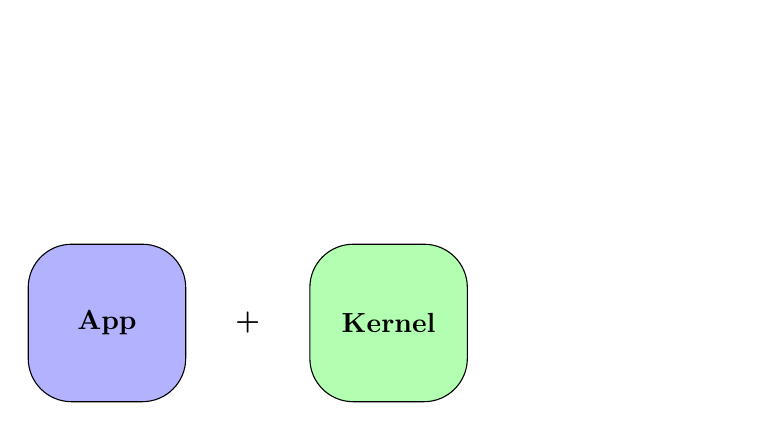
\begin{tikzpicture}[
                align=center,
                node distance=0.0cm
        ]
            \node[app] (app) {\textbf{App}};
            \node[connection, right=0.5cm of app] (plus1) {\textbf{+}};

            \node[kernel, right=0.5cm of plus1] (kernel) {\textbf{Kernel}};
            \node[connection, right=0.5cm of kernel, color=white, draw opacity=0, line width=0] (plus2) {\textbf{+}};

            \node[bpf, right=0.5cm of plus2, color=white, draw opacity=0] (bpf) {\textbf{BPF ?}};
            \node[connection, draw=none, color=white, draw opacity=0, line width=0, above=1cm of kernel] (hot-path) {Hot Path};
            \draw[arrow, draw opacity=0, line width=0, color=white, draw=none] (hot-path) to [out=60,in=90] (bpf);

        \end{tikzpicture}
    \end{center}
\end{frame}

\begin{frame}[fragile]{}
    \frametitle{}

    \begin{center}
        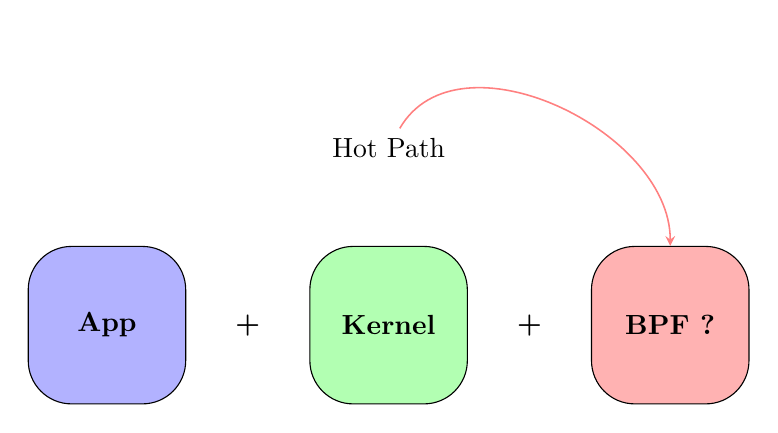
\begin{tikzpicture}[
                align=center,
                node distance=0.0cm
        ]
            \node[app] (app) {\textbf{App}};
            \node[connection, right=0.5cm of app] (plus1) {\textbf{+}};

            \node[kernel, right=0.5cm of plus1] (kernel) {\textbf{Kernel}};
            \node[connection, right=0.5cm of kernel] (plus2) {\textbf{+}};

            \node[bpf, right=0.5cm of plus2] (bpf) {\textbf{BPF ?}};
            \node[connection, above=1cm of kernel] (hot-path) {Hot Path};
            \draw[arrow] (hot-path) to [out=60,in=90] (bpf);

        \end{tikzpicture}
    \end{center}
\end{frame}

\fontsize{26pt}{26}\selectfont
\begin{frame}[fragile]{}
    \frametitle{}

    \begin{center}
        \textbf{How to measure?}
    \end{center}
\end{frame}

\fontsize{17pt}{18}\selectfont

\begin{frame}[fragile]{}
    \frametitle{Global kernel stats}

    \begin{center}
        \begin{minted}[fontsize=\Large]{shell-session}
    $ sysctl -w kernel.bpf_stats_enabled=1
    $ bpftool prog
        \end{minted}
        \vspace{0.5cm}
        \begin{minted}[fontsize=\Large]{shell-session}
    379: raw_tracepoint [...]
    run_time_ns 35875602162 run_cnt 160512637
        \end{minted}
    \end{center}
\end{frame}
\note{
    Pros: easy
    Cons: global
}

\begin{frame}[fragile]{}
    \frametitle{Good old printk}

    \begin{center}
        \begin{minted}[fontsize=\Large]{c}
    // somewhere inside your BPF prog
    bpf_trace_printk("Timestamp: %lld", ts);
        \end{minted}
        \vspace{0.5cm}
        \begin{minted}[fontsize=\Large]{shell-session}
    $ cat /sys/kernel/debug/tracing/trace_pipe
    $ bpftool prog tracelog
        \end{minted}
    \end{center}
\end{frame}
\note{
    Pros: easy, flexible
    Cons: slow, too much data
}

\begin{frame}[fragile]{}
    \frametitle{Probes before/after}

    \begin{center}
        \begin{minted}[fontsize=\Large]{shell}
    kfunc:do_syscall_64 /comm == "prog"/
    { @entry[kstack] = count(); }

    kretfunc:do_syscall_64 /comm == "prog"/
    { @return[kstack] = count(); }
        \end{minted}
    \end{center}
\end{frame}
\note{
    Pros: fast
    Cons: no ordering between progs makes it hard to find a proper point to
    attach to, maxactive, variance not relevant to the bpf prog.

    Not necessarily full syscall, maybe just before/after bpf prog.
}

\begin{frame}[fragile]{}
    \frametitle{Probes before/after}

    \begin{center}
        \begin{minted}[fontsize=\Large, escapeinside=||]{c}
  struct kretprobe {
    struct kprobe kp;
    kretprobe_handler_t handler;
    kretprobe_handler_t entry_handler;
    |\colorbox{red!20}{\textbf{int maxactive;}}|
    |\colorbox{red!20}{\textbf{int nmissed;}}|
    size_t data_size;
    struct freelist_head freelist;
    struct kretprobe_holder *rph;
  };
        \end{minted}
    \end{center}
\end{frame}
\note{
    While the probed function is executing, its return address is stored in an
    object of type kretprobe_instance.  Before calling register_kretprobe(),
    the user sets the maxactive field of the kretprobe struct to specify how
    many instances of the specified function can be probed simultaneously.
    register_kretprobe() pre-allocates the indicated number of
    kretprobe_instance objects.

mention kprobe vs kfunc, the patch and that maxactive could go away (but didn't yet).
}

\begin{frame}[fragile]{}
    \frametitle{Probes before/after}

    \begin{center}
        \begin{columns}
            \begin{column}{0.5\textwidth}
                \begin{minted}[fontsize=\large]{c}
    SEC("fentry/XXX")
    int BPF_PROG(fentry_XXX)
    {
        //...
    }
               \end{minted}
           \end{column}

           \begin{column}{0.5\textwidth}
               \begin{minted}[fontsize=\large]{c}
    SEC("fexit/XXX")
    int BPF_PROG(fentry_XXX)
    {
        //...
    }
                \end{minted}
            \end{column}
        \end{columns}
    \end{center}
\end{frame}
\note{
    Pros: fast, only target progs
    Cons: requires BTF
}

\begin{frame}[fragile]{}
    \frametitle{Probes before/after}

    \begin{center}
        \begin{minted}[fontsize=\Large]{c}
    if (!btf) {
      bpf_log(log,
        "FENTRY/FEXIT program can only be"
        "attached to another program"
        "annotated with BTF\n");
      return -EINVAL;
    }
        \end{minted}
    \end{center}
\end{frame}

\begin{frame}[fragile]{}
    \frametitle{Probes before/after}

    \begin{center}
        \begin{columns}
            \begin{column}{0.5\textwidth}
                \begin{minted}[fontsize=\large, escapeinside=||]{asm}
  |\colorbox{red!20}{\textbf{nopl   0x0(%rax,%rax,1)}}|
   xchg   %ax,%ax
   push   %rbp
   mov    %rsp,%rbp
   sub    $0x20,%rsp
               \end{minted}
           \end{column}

           \begin{column}{0.5\textwidth}
                \begin{minted}[fontsize=\large, escapeinside=||]{asm}
  |\colorbox{red!20}{\textbf{callq  0xffffffffffe0096c}}|
   xchg   %ax,%ax
   push   %rbp
   mov    %rsp,%rbp
   sub    $0x20,%rsp
                \end{minted}
            \end{column}
        \end{columns}
    \end{center}
\end{frame}
\note{
    In this way bpftool profile & perf stat -b work
}

\begin{frame}[fragile]{}
    \frametitle{Probes before/after}

    \begin{center}
        \begin{columns}
            \begin{column}{0.5\textwidth}
                \begin{minted}[fontsize=\large, escapeinside=||]{shell-session}
  $ bpftool prog profile \
      id 5 \
      duration 10 \
      cycles instructions
                \end{minted}
            \end{column}
        \end{columns}
    \end{center}
\end{frame}
\note{
    In this way bpftool profile & perf stat -b work
}

\begin{frame}[fragile]{}
    \frametitle{Profiling}

    \begin{center}
        \begin{minted}[fontsize=\large]{bash}
  Percent | uops_retired.stall_cycles
          :
          : if (duration_ns < min_duration_ns)
     0.00 :    9f:movabs $0xffffc9000009e000,%rdi
     0.00 :    a9:mov    0x0(%rdi),%rsi
          :
          : e = bpf_ringbuf_reserve(...)
    21.74 :    ad:movabs $0xffff888103e70e00,%rdi
     0.00 :    b7:mov    $0xa8,%esi
     0.00 :    bc:xor    %edx,%edx
     0.00 :    be:callq  0xffffffffc0f9fbb8
        \end{minted}
    \end{center}
\end{frame}
\note{
    Few samples, only an example. Uops_retired.stall_cycles = Cycles without
    actually retired uops.  BTF is needed, not only as debugging information,
    but also as perf facilitation.

    Sampling the whole kernel, limiting, intel_pt?
}

\fontsize{26pt}{26}\selectfont
\begin{frame}[fragile]{}
    \frametitle{}

    \begin{center}
        \textbf{How to improve?}
    \end{center}
\end{frame}

\fontsize{17pt}{18}\selectfont

\begin{frame}[fragile]{}
    \frametitle{BPF Instruction Set}

    \begin{center}
        \begin{minted}[fontsize=\large]{c}
                       if (delta < ts)
        \end{minted}

        \vspace{0.5cm}

        \begin{columns}
            \begin{column}{0.5\textwidth}
                \begin{minted}[fontsize=\large, escapeinside=||]{asm}
    ; if (delta < ts)
      cmp    %rsi,%rdi
      jae    0x0000000000000068
               \end{minted}

           \end{column}

           \begin{column}{0.5\textwidth}
                \begin{minted}[fontsize=\large, escapeinside=||]{asm}
; if (delta < ts)
  cmp    %rdi,%rsi
  jbe    0x0000000000000065
                \end{minted}

            \end{column}
        \end{columns}

    \vspace{2.0cm}
    \href{https://pchaigno.github.io/bpf/2021/10/20/ebpf-instruction-sets.html}
         {\color{links}\fontsize{10pt}{0}\selectfont eBPF Instruction Sets}
    \end{center}
\end{frame}
\note{
    Influences size of the program and final instructions (more workarounds for
    v1 here vs v2).  Wors with -mcpu=v1/v2/v3 -mattr=+alu32 (for me ‘probe’
    wasn’t working) via llc. With clang use -mllvm -mcpu …

    BPF_JLT (jump less than)
    jae (jump if above or equal, prev cmp is greater than or equal)
    jbe (jump if below or equal, prev cmp lesser than or equal)
}

\begin{frame}[fragile]{}
    \frametitle{BPF Instruction Set}

    \begin{center}
        \begin{minted}[fontsize=\Large, escapeinside=||]{shell-session}
      $ llc probe.bc
          |\colorbox{red!20}{\textbf{-mcpu=v2}}|
          |\colorbox{red!20}{\textbf{-march=+alu32}}|
          -march=bpf
          -filetype=obj
          -o probe.o
        \end{minted}
        \begin{minted}[fontsize=\Large, escapeinside=||]{shell}
      # otherwise -mllvm -mcpu=...
        \end{minted}

    \end{center}
\end{frame}
\note{
    Arithmetic logic unit
}

\begin{frame}[fragile]{}
    \frametitle{BPF 2 BPF}

    \begin{center}
        \begin{minted}[fontsize=\large]{c}
    #ifndef __inline
    # define __inline                         \
       inline __attribute__((always_inline))
    #endif
    
    static __inline int test_bpf2bpf(void) {}
        \end{minted}

        \vspace{0.5cm}

        \begin{minted}[fontsize=\large]{asm}
    # 0xffffffffc1513a68:
      nopl   0x0(%rax,%rax,1)
      xor    %eax,%eax
      push   %rbp
    # [...]
        \end{minted}
    \end{center}
\end{frame}

\begin{frame}[fragile]{}
    \frametitle{BPF 2 BPF}

    \begin{center}
        \begin{minted}[fontsize=\large]{c}
    static int test_bpf2bpf(void) { }
        \end{minted}

        \vspace{0.5cm}

        \begin{minted}[fontsize=\large]{asm}
    # 0xffffffffc15b810c:
      nopl   0x0(%rax,%rax,1)
      xor    %eax,%eax
    # [...]
      callq  0x0000000000002370

    # 0xffffffffc15ba47c:
      nopl   0x0(%rax,%rax,1)
      xchg   %ax,%ax
    # [...]
        \end{minted}
    \end{center}
\end{frame}
\note{
    Works similar to bpf helpers.
    The calling convention known from BPF helper function applies to BPF to BPF
    calls just as well, meaning r1 up to r5 are for passing arguments to the
    callee and the result is returned in r0. r1 to r5 are scratch registers
    whereas r6 to r9 preserved across calls the usual way. The maximum number
    of nesting calls respectively allowed call frames is 8. A caller can pass
    pointers (e.g. to the caller’s stack frame) down to the callee, but never
    vice versa.

    BPF JIT compilers emit separate images for each function body and later fix
    up the function call addresses in the image in a final JIT pass. This has
    proven to require minimal changes to the JITs in that they can treat BPF to
    BPF calls as conventional BPF helper calls.
}

\begin{frame}[fragile]{}
    \frametitle{BPF 2 BPF}

    \begin{center}
        \begin{minted}[fontsize=\large]{c}
  if (idx && subprog[idx].has_tail_call && depth >= 256) {
    verbose(env,
      "tail_calls are not allowed when call stack"
      "of previous frames is %d bytes. Too large\n",
      depth);
    return -EACCES;
  }
        \end{minted}
    \end{center}
\end{frame}
\note{
    protect against potential stack overflow that might happen when
    bpf2bpf calls get combined with tailcalls. Limit the caller's stack
    depth for such case down to 256 so that the worst case scenario
    would result in 8k stack size (32 which is tailcall limit * 256 =
    8k).

    To get the idea what might happen, see an example:
    func1 -> sub rsp, 128
     subfunc1 -> sub rsp, 256
     tailcall1 -> add rsp, 256
      func2 -> sub rsp, 192 (total stack size = 128 + 192 = 320)
      subfunc2 -> sub rsp, 64
      subfunc22 -> sub rsp, 128
      tailcall2 -> add rsp, 128
       func3 -> sub rsp, 32 (total stack size 128 + 192 + 64 + 32 = 416)

    tailcall will unwind the current stack frame but it will not get rid
    of caller's stack as shown on the example above.
}

\fontsize{26pt}{26}\selectfont
\begin{frame}[fragile]{}
    \frametitle{}

    \begin{center}
        \textbf{How to improve in the future?}
    \end{center}
\end{frame}

\fontsize{17pt}{18}\selectfont

\begin{frame}[fragile]{}
    \frametitle{Map batch operations}

    \begin{center}
        \begin{minted}[fontsize=\Large]{c}
    BPF_MAP_LOOKUP_BATCH
    BPF_MAP_LOOKUP_AND_DELETE_BATCH
    BPF_MAP_UPDATE_BATCH
    BPF_MAP_DELETE_BATCH
        \end{minted}
    \end{center}
\end{frame}
\note{
    aa2e93b8e58e18442edfb2427446732415bc215e
    cb4d03ab499d4c040f4ab6fd4389d2b49f42b5a5
    + Libbpf support

    Batching saves on user/kernel space interaction.
    Visible improvements ~1M records with batches of size
    10, 1000 etc.
}

\begin{frame}[fragile]{}
    \frametitle{BPF program pack allocator}

    \begin{center}
        \begin{minted}[fontsize=\Large]{c}
    struct bpf_prog_pack {
        struct list_head list;
        void *ptr;
        unsigned long bitmap[];
    };

    // [...]

    ro_header = bpf_prog_pack_alloc(
                size, bpf_fill_ill_insns);
        \end{minted}
    \end{center}
\end{frame}
\note{
    57631054fae6dcc9c892ae6310b58bbb6f6e5048
    iTLB trashing due to small progs
}

\begin{frame}[fragile]{}
    \frametitle{Bloom filter map}

    \begin{center}
        \begin{minted}[fontsize=\Large]{c}
    bpf_map_create(
        BPF_MAP_TYPE_BLOOM_FILTER, NULL,
        0, sizeof(value), 100, NULL);
        \end{minted}
    \end{center}
\end{frame}
\note{
    9330986c03006ab1d33d243b7cfe598a7a3c1baa

    A Bloom filter is a space-efficient probabilistic data structure that is
    used to test whether an element is a member of a set. False positive
    matches are possible, but false negatives are not – in other words, a query
    returns either "possibly in set" or "definitely not in set". Elements can
    be added to the set, but not removed (though this can be addressed with the
    counting Bloom filter variant); the more items added, the larger the
    probability of false positives.
}

\begin{frame}[fragile]{}
    \frametitle{Task local storage}

    \begin{center}
        \begin{minted}[fontsize=\Large]{c}
    ptr = bpf_task_storage_get(
            &start, t, 0,
            BPF_LOCAL_STORAGE_GET_F_CREATE);
        \end{minted}
    \end{center}
\end{frame}
\note{
    a10787e6d58c24b51e91c19c6d16c5da89fcaa4b

    To access per-task data, BPF programs usually creates a hash table with
    pid as the key. This is not ideal because:
     1. The user need to estimate the proper size of the hash table, which may
        be inaccurate;
     2. Big hash tables are slow;
     3. To clean up the data properly during task terminations, the user need
        to write extra logic.

	Logically, it could be thought of as getting the value from
	a *map* with *task* as the **key**.  From this
	perspective,  the usage is not much different from
	**bpf_map_lookup_elem**\ (*map*, **&**\ *task*) except this
	helper enforces the key must be an task_struct and the map must also
	be a **BPF_MAP_TYPE_TASK_STORAGE**.

	Underneath, the value is stored locally at *task* instead of
	the *map*.  The *map* is used as the bpf-local-storage
	"type". The bpf-local-storage "type" (i.e. the *map*) is
	searched against all bpf_local_storage residing at *task*.
}

\fontsize{18pt}{18}\selectfont
\begin{frame}
  \vspace*{2.5cm}
  \begin{minipage}[b][\paperheight]{\textwidth}
  \begin{center}

      %\raggedright%
      \linespread{1.0}%
      \usebeamerfont{title}%
      \usebeamercolor[fg]{title}%
      \if@noSmallCapitals%
        Questions?
      \else%
        \scshape{\color{black} Questions?}%
      \fi%
      \vspace*{0.3em}

      \usebeamerfont{subtitle}%
      \fontsize{13pt}{14}\selectfont
      \usebeamercolor[fg]{subtitle}%
        \begin{itemize}[label={}]
            \item {\color{black} \twitter\ @erthalion}
            \item {\color{black} \email\ dmitrii.dolgov at redhat dot com}
        \end{itemize}
      \vspace*{2.5em}%

    \vfill
    \vspace*{2em}
  \end{center}
  \end{minipage}
\end{frame}

\end{document}
